\documentclass[ngerman,a4paper]{report}
\usepackage[english,ngerman]{babel}
\usepackage[T1]{fontenc}
\usepackage[utf8]{inputenc}
\usepackage{geometry}
\usepackage{caption}
\usepackage{hyperref}
%\usepackage{MyriadPro}
\usepackage{graphicx}
%\geometry{verbose,tmargin=3cm,bmargin=3cm,lmargin=3cm,rmargin=3cm}
\usepackage{listings}
\usepackage{paralist}
\usepackage{stmaryrd}
\usepackage{color}
%\usepackage{floatflt}
\usepackage{amsmath}
%\usepackage{amssymb}
\usepackage{float}
\definecolor{dkgreen}{rgb}{0,0.6,0}
\definecolor{gray}{rgb}{0.5,0.5,0.5}
\definecolor{mauve}{rgb}{0.58,0,0.82}
\lstset{language=Haskell,
numbers=left,
numberstyle=\tiny\color{gray},
stepnumber=1,
numbersep=5pt,
%basicstyle=\tiny,
%frame = single,
tabsize =2,
breaklines = true,
breakatwhitespace = false,
keywordstyle=\color{blue},          % keyword style
commentstyle=\color{dkgreen},       % comment style
stringstyle=\color{mauve},         % string literal style
literate=%
{Ö}{{\"O}}1
{Ä}{{\"A}}1
{Ü}{{\"U}}1
{ß}{{\ss}}2
{ü}{{\"u}}1
{ä}{{\"a}}1
{ö}{{\"o}}1
}

%\selectlanguage{english}

\renewcommand{\familydefault}{\sfdefault}
\author{Tobias Höppner}
\title{Real World Haskell}
\date{SoSe 2013}

\begin{document}
\maketitle
\tableofcontents
\chapter{VL I}
\section{Motivation}
Warum eigentlich Haskell?\\
Haskell Compiler ist mächtig. Weil die Semantik und Typsystem wilde Sachen erlaubt. Wilde Sachen ermöglichen korrekte Software und sind meist sogar effizienter.\\

\section{Was passiert hier?! - der kleine Webserver}

\subsection{der kleine Webserver}

\lstinputlisting{code/VL/webserver.hs}

Was nicht behandelt wurde:
\begin{compactitem}
\item Fehlerfälle, Exceptions
Haskell unterstütz Exceptions 
\item Effizienz
\end{compactitem}


\subsection{Einbinden von Modulen}
import am Anfang der Datei
\begin{compactitem}
\item System.IO
\item Control.Monad (forever)
\item Text.Printf
\item Network
\item Control.Exception
\item Control.Concurrent
\end{compactitem}

\subsection{Do-Notation}
\begin{lstlisting}
main = do
	putStrLn "hallo user!!"
	putStrLn "xxxx"
	main = p "x" >> p "x"
\end{lstlisting}

ist das gleiche wie
\begin{lstlisting}
main :: IO()
main = do
	args <- getArgs
	read ((!!0) args)
	let x = read ((!! 1) args)
\end{lstlisting}

\subsubsection{Typen}

listenOn: $\_ \leftarrow \ IO\_$

\subsection{\$-Operator}
\begin{lstlisting}
f a b
\end{lstlisting}
a ist eine Fkt. g x k\\
b ist eine Fkt. k fv

\begin{lstlisting}
f $ g x k $ k f v
\end{lstlisting}

\subsection{!!-Operator}
Gibt das angegebene Element aus der Liste zurück.
\begin{lstlisting}
(!!) :: [a] -> Int -> a
let xs = []
ys = [1,2,4]
zs = [1..1378]

zs !! 0
\end{lstlisting}
\section{der größere Webserver}
%code einbinden

\section{builds}
\subsection{mit ghc}
\begin{lstlisting}
ghc x.hs
\end{lstlisting}
Wird unübersichtlich für mehrere Dateien / Module.

\subsection{mit cabal}
\begin{lstlisting}
cabal configure
cabal build
cabal install
\end{lstlisting}

Projekte werden als \textbf{.cabal} gespeichert, sind eleganter und man kann schneller testen.

\section{.(Punkt)-Operator}
\begin{lstlisting}
(.):: (b -> c) -> (a -> b) -> (a -> c)
f . g
\end{lstlisting}

entspricht\\

\begin{lstlisting}
(\x -> f ( g x))
\end{lstlisting}

\section{Generics in Haskell}

\begin{lstlisting}
List e
m k v
\end{lstlisting}

\section{Stdlib - System.IO}
\begin{compactitem}
\item Textinput / Textoutput
\begin{compactitem}
\item Print
\item getLine
\item getChar
\end{compactitem}
\end{compactitem}

\section{Stdlib - System.Environment}
\begin{compactitem}
\item getArgs
\end{compactitem}

\section{Kommentare und Haddock}
\begin{lstlisting}
-- einfacher Kommentar
{- mehrzeiliger Kommentar -}
{- mehrzeiliger Kommentar 
	{- verschachtelter Kommentar -} 
-}
-- | haddoc kommentar
\end{lstlisting}

\section{Keywords}
Programming Guidelines sind brauchbar
\begin{lstlisting}
main = do 
	args <- getArgs
	case args of
		[] -> ...
		["-x"] -> ...
		["-x",b] -> ...
\end{lstlisting}

\chapter{VL II}
\section{Zustände in Haskell}
Gestern wurde der Taschenrechner implementiert, heute sehen wir uns an wie man die eval-Funktion weiter entwickeln kann.
\subsection{Eval Funktion in "besser"}
\begin{lstlisting}
data Expr = Const Float | Add Expr Expr | Div Expr Expr

eval0 :: Expr -> Float
eval0 (Const x) = x = id x
eval0 (Add e1 e2) = evalO(e1) + evalO(e2)
eval0 (Div e1 e2) = evalO(e1) / evalO(e2)
eval0 (Div (Const 1) (Const 0)) = Infinity
\end{lstlisting}
Zunächst abstrahieren wir das pattern matching mithilfe einer neuen Funktion \textbf{evalExpr}. Die Hilfsfunktionen \textbf{fC}, \textbf{fA}, \textbf{fD} stehen jeweils für das ermitteln einer Konstanten, das Berechnen einer Addition oder das Berechnen einer Division.
\begin{lstlisting}
fC :: Float -> Float
fA :: Float -> Float -> Float
fD :: Float -> Float -> Float

evalExpr fC fA fD (Const x) = fC x
evalExpr fC fA fD (Add e1 e2) = fA (evalExpr fC fA fD e1) (evalExpr fC fA fD e2)
evalExpr fC fA fD (Div e1 e2) = fD (evalExpr fC fA fD e1) (evalExpr fC fA fD e2)
\end{lstlisting}
Eine Fehlerbehandlung kann wie folgt realisiert werden:
\begin{lstlisting}
eval1 = eval Expr id (+) fD
	where fD x y = if y == 0 then error "div by 0!" else (x/y)
\end{lstlisting}
Hier wird das Programm mit \textbf{error} abgebrochen sobald der Wert $0$ für $y$angegeben wird. Besser wäre es eine Funktion zu formulieren die einen zusätzlichen Fehlerwert ausgeben kann (\textbf{Nothing}). Alle erfolgreichen Ergebnisse sind in ein \textbf{Just} verpackt.\\
Zur Erinnerung \textbf{Maybe} ist wie folgt definiert:
\begin{lstlisting}
data Maybe a = Nothing | Just a
\end{lstlisting}
In unserem Fall hat \textbf{Just} folgende Signatur:
\begin{lstlisting}
Just :: Float -> Maybe Float
\end{lstlisting}
Damit kann man jetzt eine bessere \textbf{Eval-}Funktion schreiben:
\begin{lstlisting}
eval2 :: Expr -> Maybe Float
eval2 = evalExpr Just fA fD
	where
		fA e1 e2 = case e1 of
			Nothing -> Nothing
			Just x -> case e2 of
				Nothing -> Nothing
				Just y -> Just (x + y)
		fD e1 e2
			Nothing -> Nothing
			Just x -> case e2 of
				Nothing -> Nothing
				Just y -> Just (x / y)
\end{lstlisting}
\subsection{Abstrahieren}
\textbf{fA} und \textbf{fD} folgen dem selben Muster:
\begin{lstlisting}
func x ... = case x of
	Nothing -> Nothing
	Just x -> ... some stuff with x ...
\end{lstlisting}
Mit dieser Erkenntnis können wir eine weitere Hilfsfunktion definieren \textbf{op}:
\begin{lstlisting}
op :: Maybe a -> (a -> Maybe b) -> Maybe b
op val f = case val of
	Nothing -> Nothing
	Just x -> f x
\end{lstlisting}
Die Funktion \textbf{f} überführt einen Wert vom Typ $a$ in ein $Maybe b$. \textbf{op} betrachtet das Argument $val$ und wendet entweder \textbf{f} auf den in \textbf{Just} verpackten Wert an, oder gibt \textbf{Nothing} zurück.
\begin{lstlisting}
eval3 = eval Expr Just fA fD
	where 
		fA e1 e2 = e1 'op' (\x -> e2 'op' (\y -> (x + y)))
		fA e1 e2 = e1 'op' (\x -> e2 'op' (\y -> (x / y)))
\end{lstlisting}

Der Taschenrechner von gestern hat jetzt eine Fehlerbehandlung die das Programm nicht abbricht, sondern eine adequate Fehlerbehandlung durchführt. (Fehlerhafte Werte werden mit \textbf{Nothing} symbolisiert.\\

\section{Zustandsveränderung}

%Bild state_trans1.png
\begin{figure}[h]
	\centering
	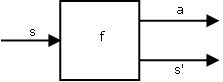
\includegraphics[width=150px]{gfx/state_trans1.png}
	\caption{Zustandsveränderungen}
	\label{img:statetrans}
\end{figure}

Taschenrechner können sich meist Werte für verschiedene Variablen oder das letzte Ergebenis merken. Wir versuchen hier letzteres zu speichern:
\begin{lstlisting}
type State = Float
\end{lstlisting}
\textbf{type} deklariert ein Type-Alias.\\

Jetzt brauchen wir eine Funktion die zustandsveränderungen konkret behandeln kann. Quasi als eine Art Objekte (keine OOP-Objekte).
\begin{lstlisting}
update :: Float -> State -> State
update f = max abs(f)

data St a = S(State -> (a,State))
\end{lstlisting}

"Folgezustand" berechnen

\begin{lstlisting}
apply :: St a -> State -> (a, State) -- Startzustand -> (Ergebnis und Folgezustand)
appl (S f) s = f s
\end{lstlisting}

Unterschied data / type Listings:\\
\textbf{type} beschreibt wie man einen Zustand definiert.
\textbf{data} beschreibt wie man einen Zustand verändert.

\subsection{Verbesserte Eval-Funktion}
\begin{lstlisting}
eval4 :: Expr -> St Float
eval4 = eval Expr fC fA fD
	where
		fC x = S (\s -> (x,s))
		fA sx sy = S (\s -> let (x, s1) = apply sx s
									(y, s2) = apply sy s1
								in (x + y, update(x+y) s2))
		fA sx sy = S (\s -> let (x, s1) = apply sx s
									(y, s2) = apply sy s1
								in (x / y, update(x/y) s2))
\end{lstlisting}
Man erkennt, hier kann man \textbf{apply} durch eine neue Funktion \textbf{ap} verkürzen:
\begin{lstlisting}
ret x = S (\s -> (x,s))

ap:: St a -> (a -> St b) -> St b
ap st f = S (\s -> let (x, s1) = apply st s
						in apply (f x) s1)

eval5 = evalExpr fC fA fD
	where
		fC x = ret x
		fA sx sy = sx 'ap' (\x ->
					sy 'ap' (\y ->
					s(\s -> (x+y, update abs (x+y) s))))
		fD sx sy = sx 'ap' (\x ->
					sy 'ap' (\y ->
					s(\s -> (x/y, update abs (x/y) s))))
\end{lstlisting}

\subsection{Zustände nutzen}
Damit wir die Zustände auch verwenden können müssen wir sie auslesen und manipulieren können:
\begin{lstlisting}
get :: St State
get = S (\s -> (s,s))

put :: State -> St ()
put s = S(\_ -> ((),s))
\end{lstlisting}

Unsere neue \textbf{Eval}-Funktion sieht danach so aus:

\begin{lstlisting}
stAct :: (State -> State) -> St ()
stAct f = get 'ap' (put.f)

eval6 = evalExpr fC fA fD
	where
		fC = ret
		fA sx sy = sx 'ap' (\x ->
					sy 'ap'	 (\y -> 
					stAct (update(x+y)) 'ap' (\() -> ret (x+y)))))
		fD sx sy = sx 'ap' (\x ->
					sy 'ap'	 (\y -> 
					stAct (update(x\y)) 'ap' (\() -> ret (x\y)))))
\end{lstlisting}

Man sollte erkennen das es immer wieder gleiche Muster gibt. Dieses Muster tritt so häufig in der funktionalten Programmierung auf, dass man es in eine einheitliche Schnittstelle verpackt hat.
\section{Monaden}
\begin{lstlisting}
class Monad m where
	return :: a -> m a
	(>>=)	:: m a -> (a -> m b) -> m b
\end{lstlisting}
\textbf{ap} ist eine Monade!\\
In Haskell schreibt man das so:
\begin{lstlisting}
instance Monad Maybe where
	return = Just
	(>>=) = op
\end{lstlisting}

\subsection{die letzte Eval-Funktion (wirklich!)}
So implementiert man ungefähr immer eine Monade, \textbf{eval3}, \textbf{eval5} und \textbf{eval6} lassen sich so vereinfachen:
\begin{lstlisting}
evalM :: Monad m => Expr -> m Float
evalM = eval Expr fC fA fD
	where
		fC = return
		fA m1 m2 = m1 >>= (x -> 
					m2 >>= (y ->
						... -- irgendwas spezifisches
						return (x+y))))
		fD m1 m2 = m1 >>= (x -> 
					m2 >>= (y ->
						if y == 0 -- irgendwas spezifisches
						then Nothing
						else return (x/y))))
\end{lstlisting}
Für
\begin{lstlisting}
m >>= \x -> fx
\end{lstlisting}
schreibt man auch
\begin{lstlisting}
do x <- m
	return (f x)
\end{lstlisting}

Und
\begin{lstlisting}
m1 >> m2
\end{lstlisting}
ist nichts anderes als
\begin{lstlisting}
do	m1
		m2
\end{lstlisting}

Für Monaden gibt es 3 Gesetze, die stehen in der Doku.

\chapter{VL III}
\section {Wiederholung Monanden}
Wir definieren uns unsere eigene Monade, dazu brauchen wir einen Datentyp:
\begin{lstlisting}
data Entweder a = Links String | Rechts a
\end{lstlisting}

Zur Erinnerung, Monaden sind wie folgt typisiert
\begin{lstlisting}
class Monad m where
	return :: a -> m a
	(>>=) :: m a -> (a -> m b) -> m b
	(>>) :: m a -> m b -> m b
	fail :: String -> m a
\end{lstlisting}

implementieren kann man das so:

\begin{lstlisting}
instance Monad Entweder where
	return = Rechts 
	m >>= f = case of
		Rechts wert -> f wert
		_ -> m
	m >> n = case of
		Rechts _ -> n
		Links message -> Links message 
	fail str = Links str
\end{lstlisting}

Im Grunde braucht man nur \textbf{return} und \textbf{(>>=)}(bind). \textbf{(>>)} und \textbf{fail} sind nettigkeiten die uns das Leben in bestimmten Situationen vereinfachen können. Es gibt stimmen die behaupten, man braucht diese Funktionen nicht und man könnte diese auch durch eine extra Monade darstellen.\\

\subsection{Maybe Monad}
\begin{lstlisting}
instance Monad Maybe where
	return Just
	m >>= f = case m of
		Just wert -> f wert
		_ -> Nothing
	fail _ = Nothing
\end{lstlisting}

Wie verwendet man diese Monade?

\begin{lstlisting}
f :: Int -> Maybe k
f i = if i == 0 then Nothing else Just i
\end{lstlisting}

kann man mit der \textbf{Maybe} Monade auch so schreiben:
\begin{lstlisting}
f i = if i == 0 then fail "not 0" else return i
\end{lstlisting}
Nice to know: Listen in Haskell sind auch Monaden.

\subsection{Die Id-Monade}
\begin{lstlisting}
data Id a = Id a
\end{lstlisting}

\begin{lstlisting}
instance Monad Id where
	return = Id 
	(ID x) >>= f = f x 
\end{lstlisting}

Warum braucht man die?
Wir kennen die Id-Funktion
\begin{lstlisting}
id :: a -> a
id x = x
\end{lstlisting}

Für die Monaden gibt es noch keine ID Funktion. Deswegen definiert man sich die wie folgt:

\begin{lstlisting}
id :: Monad m => a -> Id a
id x = return
\end{lstlisting}

Haskell kennt 2 Welten, alles ohne Monaden und alles mit Monaden. 
Beispiele:
Ohne Monaden:
\begin{compactitem}
\item id
\item map
\item ...
\end{compactitem}
Mit Monaden:
\begin{compactitem}
\item return
\item mapM
\item ...
\end{compactitem}

\subsubsection{Beispiel funktionale For-Schleife}

\begin{lstlisting}
print :: Show a => a IO ()

main :: IO()
main = do
	let xss = ["Hallo", "Welt", "da draußen"]
	mapM print xss
\end{lstlisting}

oder auch direkt mit \textbf{forM}

\begin{lstlisting}
forM :: [a] -> (a -> m b) -> m [b]

main = do
	let xss = ["Hallo", "Welt", "da draußen"]
	forM xss $ do
		...	-- irgendwas
		...	-- irgendwas anderes
		...	-- irgendwas weiteres
	putStrLn "xxx"
\end{lstlisting}

Wie ist \textbf{forM} implementiert?

\begin{lstlisting}

\end{lstlisting}

\section{Die IO-Monade}
Bereits eine Ausgabe auf eine Konsole ist ein Seiteneffekt. In Haskell ist man aber eher exakt und möchte Seiteneffekte vermeiden. Dafür gibt es die IO-Monade, der Ansatz:
\begin{lstlisting}
main :: [Response] -> [Request]
main (x:xs) = Print "Hello World" : main xs
\end{lstlisting}
Das ist ziemlich umständlich zu implementieren. Wurde trotzdem in Haskell 1.3 vorgeschlagen. Wie können wir jetzt elegant die Haskell-Welt verlassen? Richtig mit der IO-Monade:
\begin{lstlisting}
main :: IO()
main = do
	map print [8,9,9] 	--> [IO, IO, IO]
	mapM print [8,9,9] 	-->	8
											--	9
											--	9
\end{lstlisting}
Die IO-Monade ist eine State-Monade. Die macht noch etwas mehr "magic" damit man "sauber" mit dem OS komunizieren kann.\\
Monaden sind sehr mächtig. Man kann sich mit Monaden zwingen bestimmte Dinge nicht zu tun. Das ist hilfreich und gerade wenn man Monaden miteinander verbindet. Der Vorteil von Haskell ist gerade, das man mit Monaden zu bestimmten Situationen Seiteneffekte ausschliessen kann. Das ist gerade für "sichere" Software interessant.\\

\section{Arbeiten mit Monaden}
\subsection{Das Echo}
\begin{lstlisting}
module Main where
-- putStr :: String -> IO()
-- putStrLn :: String -> IO()
-- print :: Show a => a -> IO()
-- getLine :: IO String

main :: IO()
main = do
	line <- getLine
	putStrLn line
	-- main -- für endlosschleife, alternativ zu main = forever $ do
-- main = getLine >>= putStrLn

main = forever (getLine >>= putStrln) -- cat in einer Zeile
\end{lstlisting}

\subsection{handles}
Werden meist von anderen Funktionen übergeben. Man kann Handels mit entsprechenden h.. Funktionen.
\begin{lstlisting}
module Main where
-- hputStr :: Handle -> String -> IO()
-- hputStrLn :: Handle -> String -> IO()
\end{lstlisting}

\section{Gloss}
Gloss ist echtes, extrem vereinfachtes OpenGL. Einfaches Beispiel: 
\begin{lstlisting}
import Graphics.Gloss

main = display(InWindow "Nice Window" (200,200) (10,10)) white (Circle 80))
\end{lstlisting}
GHCi mag nicht unbedingt Gloss. Also erstmal bauen und dann ausführen.\\

\subsection{komplexere Bilder}
Wie zeichne ich ein komplexes Bild?\\
\begin{lstlisting}
import Graphics.Gloss

main = display
	(FullScreen (1280,800)) 
	black
	(
		Pictures[
			Translate (-200) 0 (Color red (Circle 100)),
			Translate 100 0 (Color yellow (Circle 100)),
			Color white (ThickCircle 100 200),
			Translate 100 100 $ Color blue $ Circle 300
		]		
	) 
\end{lstlisting}
toll ist: man kann in Pictures einfach funktionen übergeben, die Funktionen sollte man natürlich vorher definieren. Das macht den Code lesbarer.
\begin{lstlisting}
redCircle = Color red $ Cricle 100
yellowCircle = Color yellow $ Circle 100
whiteCircle = Color white $ Circle 200

main' = display
	(FullScreen (1280,800)) 
	black
	(
		Pictures[
			Translate (-200) 0 redCricle,
			Translate 100 0 yellowCircle,
			whitecircle,
			Translate 100 100 $ Color blue $ Circle 300
		]		
	)
\end{lstlisting}

Der Bildmittelpunkt ist entscheidend. $0,0$ ist der Mittelpunkt des Bildschirms.

\subsection{Animationen}
\begin{lstlisting}
main = animate
	(InWindow "Titel" (400, 300) (100, 100))
	white
	\t -> (Pictures)
\end{lstlisting}

\end{document}
